\section{尖点的产生}
\label{sec:hj-cusps}

定理~\ref{thm:hj-local-classical}只保证短时间内有解。时间一长，映射$\bm{y}\mapsto\bm{x}(\bm{y},t)$可能不再可逆，同一个位置会被几条特征线到达。这时经典解到了尽头，而且仅仅要求方程几乎处处成立，也无法决定接下来该怎么办。

\paragraph{梯度沿特征线的变化}
取$d=1$，$H=H(p)$。此时$\dot{p}=-\partial_xH=0$，斜率沿特征线不变，特征线是直线：
\[
  x(y,t)=y+tH'\bigl(u_0'(y)\bigr).
\]
对$y$求导，记$a(y)=H''(u_0'(y))\,u_0''(y)$，得到
\[
  \partial_yx=1+ta(y).
\]

二阶导数$w=\partial_x^2u$沿特征线的取值，可以用$\partial_yp/\partial_yx$算出。由$p=u_0'(y)$，
\begin{equation}
  w(y,t)=\frac{u_0''(y)}{1+ta(y)}.
  \label{eq:hj-riccati}
\end{equation}
若$H$是严格凸的，$a(y)<0$恰好发生在$u_0''(y)<0$的地方，也就是初值向下弯的地方。这些地方的分母随时间减小，到$t=-1/a(y)$时变成零，曲率发散。

\begin{theorem}[经典解的首次失效]
\label{thm:hj-breakdown}
设$d=1$，$H\in C^2$，$u_0\in C^2$，且$u_0'$、$u_0''$有界，$H''$在$u_0'$的值域上有界。记$m=\inf_ya(y)$。

若$m\geq0$，令$t^*=\infty$；若$m<0$，令$t^*=-1/m$。则在$0\leq t<t^*$上，$y\mapsto x(y,t)$是$\mathbb{R}$到$\mathbb{R}$的同胚，特征线给出整个$\mathbb{R}\times[0,t^*)$上的$C^2$解。若$m<0$且下确界在某点$y^*$处达到，则
\begin{equation}
  \lim_{t\uparrow t^*}\bigl\lvert\partial_x^2u(x(y^*,t),t)\bigr\rvert=\infty,
  \label{eq:hj-breakdown}
\end{equation}
所以这个解不能在$t^*$之后作为$C^2$解延拓。
\end{theorem}

\begin{proof}
设$0\leq t<t^*$。此时
\[
  \partial_yx=1+ta(y)\geq1+tm\geq\kappa>0,
\]
其中$m\geq0$时取$\kappa=1$，$m<0$时取$\kappa=1-t/t^*$。一阶导数有正下界，所以$y\mapsto x$严格递增，并且$\lvert x\rvert\to\infty$（$\lvert y\rvert\to\infty$时），是同胚。

在每个闭区间$[0,t_2]\subset[0,t^*)$上，$\kappa$有统一的正下界。逐点应用定理~\ref{thm:hj-local-classical}的计算，得到连续可微的$u$，且$\partial_xu=p$。由$w$的公式，$\partial_xu$关于$x$连续可微，$u$是$C^2$解。

式~\eqref{eq:hj-breakdown}由式~\eqref{eq:hj-riccati}得到：在$y=y^*$处，分母是$1+tm=1-t/t^*\to0$，分子$u_0''(y^*)$不为零（因为$a(y^*)=m<0$）。若存在$C^2$延拓，$\partial_x^2u$在紧集上有界，这与发散矛盾。
\end{proof}

定理说的是：斜率的变化率在有限时间内发散，而斜率和场值本身一直有界。这和第~\ref{chap:scalar-conservation-laws}章的结论对应，$v=\partial_xu$正是在同一时刻由光滑变成间断。

把定理用到例~\ref{ex:hj-cos}。$a(y)=u_0''(y)=-\cos y$，最小值$-1$在$y=0$处取得，所以$t^*=1$。特征线和曲率是
\[
  \partial_yx=1-t\cos y,\qquad w=\frac{-\cos y}{1-t\cos y}.
\]
在$x=0$（$y=0$）处，$w=-1/(1-t)$。$t=0.5$时曲率是$-2$，$t=0.9$时是$-10$。图~\ref{fig:hj-cos-steepening}显示$u$在原点越来越尖，斜率曲线越来越陡。

\begin{BookInlineFigure}
  \centering
  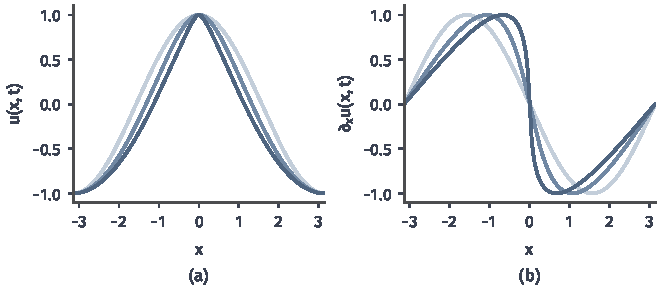
\includegraphics[width=112mm]{figures/06-differential-equations/02-partial-differential-equations/matplotlib/hj-cos-steepening/figure.pdf}
  \caption{$H=p^2/2$、$u_0=\cos x$的经典解，蓝色由浅到深是$t=0,0.5,0.9$。(a)场值$u$。(b)斜率$\partial_xu$，$x=0$处的斜率变化率是$-1/(1-t)$，$t\uparrow1$时发散，而斜率一直保持在$[-1,1]$内。}
  \label{fig:hj-cos-steepening}
\end{BookInlineFigure}

图~\ref{fig:hj-cos-characteristics}(a)把特征线全部画出来。$t<1$时它们互不相交，$t=1$时最先在红点相遇。条件$\partial_yx=0$给出特征线族的包络
\[
  t=\frac{1}{\cos y},\qquad x=y-\tan y,
\]
即图中的深灰曲线，称为\term{焦散线}（caustic）。两支焦散线之间的每个点都有三条特征线经过，这个区域由红点向上张开。

\begin{BookInlineFigure}
  \centering
  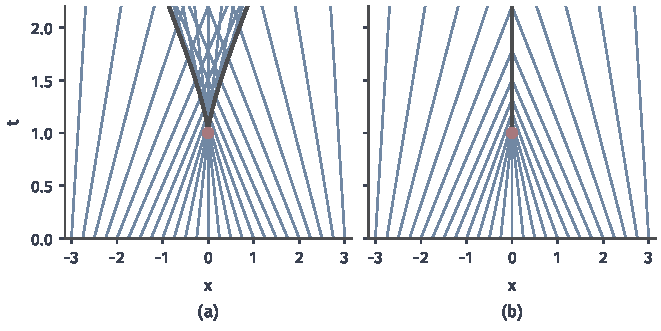
\includegraphics[width=112mm]{figures/06-differential-equations/02-partial-differential-equations/matplotlib/hj-cos-characteristics/figure.pdf}
  \caption{$u_0=\cos x$的特征线$x=y-t\sin y$（蓝）。(a)全部画出，它们在红点$(0,1)$首次相遇，深灰曲线是焦散线。(b)只画到撞上$x=0$（深灰粗线）为止的部分，第~\ref{sec:hj-hopf-lax}节将说明解用到的正是这一部分。}
  \label{fig:hj-cos-characteristics}
\end{BookInlineFigure}

\paragraph{同一位置的多个分支}
$t^*$之后，公式仍然能算，只是不再给出函数。取$t=\pi/2$、$x=0$，要求解
\[
  y=\frac{\pi}{2}\sin y.
\]
它有三个解$y=0$、$y=\pi/2$、$y=-\pi/2$。代入$p=-\sin y$和$z=\cos y+\frac{t}{2}\sin^2y$，得到
\[
  \begin{gathered}
    y=0:\quad(p,z)=(0,1),\\
    y=\tfrac{\pi}{2}:\quad(p,z)=(-1,\tfrac{\pi}{4}),\\
    y=-\tfrac{\pi}{2}:\quad(p,z)=(1,\tfrac{\pi}{4}).
  \end{gathered}
\]
三条特征线带来三对不同的斜率和值，$u(0,\pi/2)$应当取哪一个？特征方程组只负责沿线传递，回答不了这个问题。

图~\ref{fig:hj-swallowtail}(a)是$t=\pi/2$时$(x,z)$的像。曲线在$\lvert x\rvert\leq0.33$内折叠成三层，整条曲线不是函数图像。图(b)是相平面上$(x,p)$的像，初始的正弦曲线被Hamilton流剪切后折叠，同一个$x$上有三个$p$。蓝色画的是后面选出的解，下包络在$x=0$处有折角，斜率从$+1$跳到$-1$。

\begin{BookInlineFigure}
  \centering
  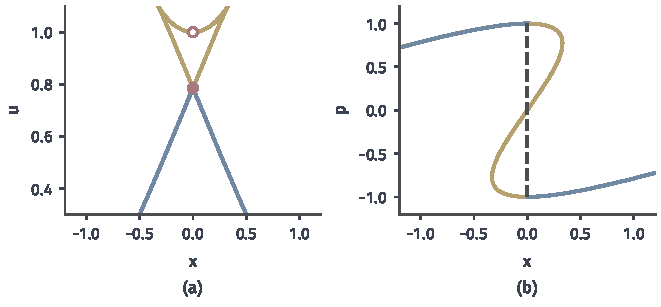
\includegraphics[width=112mm]{figures/06-differential-equations/02-partial-differential-equations/matplotlib/hj-swallowtail/figure.pdf}
  \caption{$t=\pi/2$时的多值像（黄）与选出的解（蓝）。(a)$(x,z)$平面，$x=0$处有三个值，红点是$\pi/4$（两条分支的公共值），空心点是$1$。(b)$(x,p)$平面，折叠的曲线在$x=0$处被虚线截断，蓝线在$x=0$处从$p=1$跳到$p=-1$。}
  \label{fig:hj-swallowtail}
\end{BookInlineFigure}

到达时间问题里，这个选择有明确的物理含义。平面上有两个源$\bm{a}=(-1,0)$和$\bm{b}=(1,0)$，时刻$0$同时点燃。每个源单独产生的到达时间是$T_1=\lVert\bm{x}-\bm{a}\rVert_2$和$T_2=\lVert\bm{x}-\bm{b}\rVert_2$，都是经典解。但一点只会被第一次到达的波前扫到，所以
\[
  T=\min\{T_1,T_2\}.
\]
后到的波前经过的是已经扫过的区域，没有意义。

图~\ref{fig:hj-two-sources}(a)显示两列圆形波前相遇后在中垂线上消失，$T$沿这条线不可微。在直线$x_2=1$上看，两条分支在$x_1=0$处都等于$\sqrt2$，斜率分别是$+1/\sqrt2$和$-1/\sqrt2$，取最小值后在该点形成折角，见图(b)。

\begin{BookInlineFigure}
  \centering
  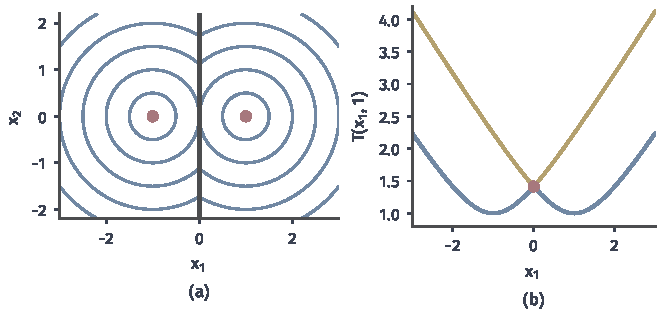
\includegraphics[width=112mm]{figures/06-differential-equations/02-partial-differential-equations/matplotlib/hj-two-sources/figure.pdf}
  \caption{两个同时点燃的源（红点）。(a)蓝线是$T=\min\{T_1,T_2\}$的等值线，深灰线是中垂线，两列波前在此相遇后消失。(b)沿$x_2=1$的截面，黄线是两个单独的到达时间，蓝线是取最小值的结果，红点是折角，高度$\sqrt2$。}
  \label{fig:hj-two-sources}
\end{BookInlineFigure}

这两个例子都选了较小的值。这究竟是巧合，还是方程本身的要求？下面的例子说明，光凭几乎处处的逐点检验回答不了。

\paragraph{几乎处处满足方程仍然不够}
取$H=p^2/2$，$u_0=0$。$u\equiv0$满足方程和初值。还有没有别的连续解？令
\begin{equation}
  w(x,t)=\min\Bigl\{\lvert x\rvert-\frac{t}{2},\ 0\Bigr\}.
  \label{eq:hj-notch}
\end{equation}
它的形状是一个越挖越深的凹槽，在$\lvert x\rvert\geq t/2$上等于$0$，在$\lvert x\rvert<t/2$上等于$\lvert x\rvert-t/2$。

逐块验证。在$\lvert x\rvert>t/2$上$w=0$，方程成立。在$0<\lvert x\rvert<t/2$上$\partial_xw=\pm1$，$\partial_tw=-1/2$，所以
\[
  \partial_tw+\frac12(\partial_xw)^2=-\frac12+\frac12=0.
\]
除了三条线$x=0$、$x=\pm t/2$，方程都成立，这三条线的测度为零。初值也满足。于是$w$和$0$是同一个初值问题的两个几乎处处解，见图~\ref{fig:hj-notch}(a)。

图~\ref{fig:hj-notch}(b)把凹槽翻译成斜率。$v=\partial_xw$在$x=\pm t/2$处的跳跃满足Rankine--Hugoniot条件，例如$x=t/2$处左值$1$、右值$0$，通量$v^2/2$给出速度$1/2$。而在$x=0$处，$v$从$-1$跳到$+1$，这是左值小于右值的间断。第~\ref{chap:scalar-conservation-laws}章的熵条件说，凸通量下的间断必须左值大于右值，否则特征线会从间断面向外分开。$x=0$处的跳跃正好违反这一条。

\begin{BookInlineFigure}
  \centering
  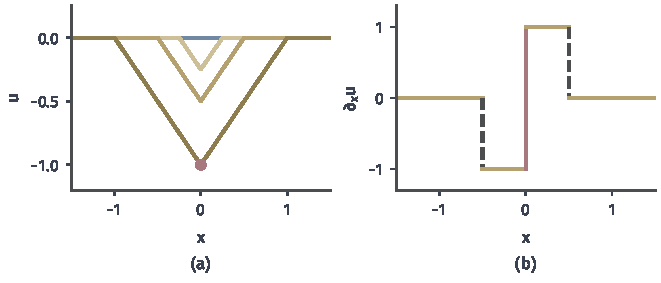
\includegraphics[width=112mm]{figures/06-differential-equations/02-partial-differential-equations/matplotlib/hj-notch/figure.pdf}
  \caption{初值为$0$时的非唯一性。(a)蓝线是$u=0$，黄色由浅到深是式~\eqref{eq:hj-notch}的$w$在$t=0.5,1,2$的图像，红点是底部折角。(b)$t=1$时的斜率$\partial_xw$，深灰虚线处的跳跃左值大于右值，红线处的跳跃左值小于右值。}
  \label{fig:hj-notch}
\end{BookInlineFigure}

因此，光用“几乎处处”这条标准，经典解失效后方程给不出答案。需要在不可微的点上也提出要求，而且要求必须能区分$w$底部的折角和$T$的尖峰。这是下一节的任务。
